% Included from both -slides and -handout versions.
%
% TODO:
%
% Next year, move 'trap' intro slide from lecture 3 to this lecture.
%
% Something about blocking vs. non-blocking system calls?

\mode<presentation>
{
  \usetheme{default}
  \useoutertheme{infolines}
}

\usepackage[english]{babel}
\usepackage[latin1]{inputenc}
\usepackage{graphicx}
\usepackage{times}
\usepackage[T1]{fontenc}
\usepackage{fancyvrb}
\usepackage{listings}
\usepackage{multirow}
\usepackage{ulem}
\begin{document}
\lstset{language=C, escapeinside={(*@}{@*)}, numbers=left,
  basicstyle=\tiny, showspaces=false, showtabs=false}

\title{L41 - Lecture 4: The Process Model (2)}
%\institute{University of Cambridge}
%\author{George V. Neville-Neil}
\author{Dr Robert N. M. Watson}
\date{3 November 2015}

\begin{frame}
  \titlepage
\end{frame}

\section{Introduction}

\begin{frame}
  \frametitle{Reminder: last time}

  \begin{enumerate}
    \item The process model and its evolution
    \begin{itemize}
      \item \textit{Isolation} via \textit{virtual addressing} and
	\textit{rings}
      \item \textit{Controlled transition} to kernel via \textit{traps}
      \item \textit{Controlled communication} to other processes via the kernel
    \end{itemize}
    \item Brutal introduction to virtual memory
    \item Programs: \textit{ELF} and \textit{run-time linking}
  \end{enumerate}
\end{frame}

\begin{frame}
  \frametitle{This time: more about the process model}

  \begin{enumerate}
    \item More on traps and system calls
    \begin{itemize}
      \item Synchrony and asynchrony
      \item Security and reliability
      \item Entry and return
    \end{itemize}
    \item Virtual memory support for the process model
    \item \sout{Threads and the process model}
    \item Readings for next time
  \end{enumerate}
\end{frame}

\section{System calls}

\begin{frame}
  \frametitle{System calls}

  \begin{itemize}
    \item User processes request kernel services via \textit{system calls};
      e.g.,
    \begin{itemize}
      \item \texttt{open()} opens a file and returns a file descriptor
      \item \texttt{fork()} creates a new process
    \end{itemize}

    \pause
    \medskip

    \item System calls exposed via library functions (e.g., in
      \texttt{libc})
    \begin{itemize}
      \item Function triggers \textit{trap} to transfer control to the kernel
      \item Arguments and return values copied in/out of kernel
      \item Kernel returns control to userspace once done
    \end{itemize}

    \pause
    \medskip

    \item Some quirks relative to normal APIs; e.g.,
    \begin{itemize}
      \item C return values via normal ABI calling convention...
      \item ... but also per-thread \texttt{errno} to report error conditions
      \item ... \texttt{EINTR}: for some calls, work got interrupted, try again
    \end{itemize}
  \end{itemize}
\end{frame}

\begin{frame}
  \frametitle{System-call synchrony}

  \begin{itemize}
    \item Some syscalls manipulate control flow or process/thread life cycle
    \begin{itemize}
      \item \texttt{\_exit()} never returns
      \item \texttt{fork()} returns ... twice
      \item \texttt{pthread\_create()} creates a new thread
    \end{itemize}

    \pause
    \medskip

    \item But most syscalls behave like C functions and are \textit{synchronous}
    \begin{itemize}
      \item Called with arguments (by value, by reference)
      \item Return values (an integer/pointer, or by reference)
      \item When the caller regains control, the work is done
      \item \texttt{getpid()} retrieves the \textit{process ID} via return value
      \item \texttt{read()} reads data from a file: on return, data is in buffer
    \end{itemize}
  \end{itemize}
\end{frame}

\begin{frame}
  \frametitle{System-call asynchrony}

  \begin{itemize}
    \item However, synchronous syscalls often perform \textit{asynchronous} work
    \begin{itemize}
      \item Some types of work may not be complete on system-call return

      \pause
      \smallskip

      \item \texttt{write()} writes data to a file .. goes to disk eventually
      \item Caller can re-use buffer immediately (`copy semantics`)

      \pause
      \smallskip

      \item \texttt{mmap()} maps a file but doesn't load data
      \item Caller will trap on attempted access; trigger actual I/O
    \end{itemize}

    % Next year, something about blocking/non-blocking calls here?

    \pause
    \medskip

    \item Some syscalls are explicitly asynchronous
    \begin{itemize}
      \item \texttt{aio\_write()} explicitly requests an asynchronous write
      \item Calls to \texttt{aio\_return()}/\texttt{aio\_error()} collect
	results later
      \item Caller must wait to re-use buffer (`shared semantics`)
    \end{itemize}
  \end{itemize}
\end{frame}

\begin{frame}
  \frametitle{System-call invocation from user to kernel}

  \begin{columns}[T]
    \column{.35\textwidth}
      \vspace{0.25cm}
      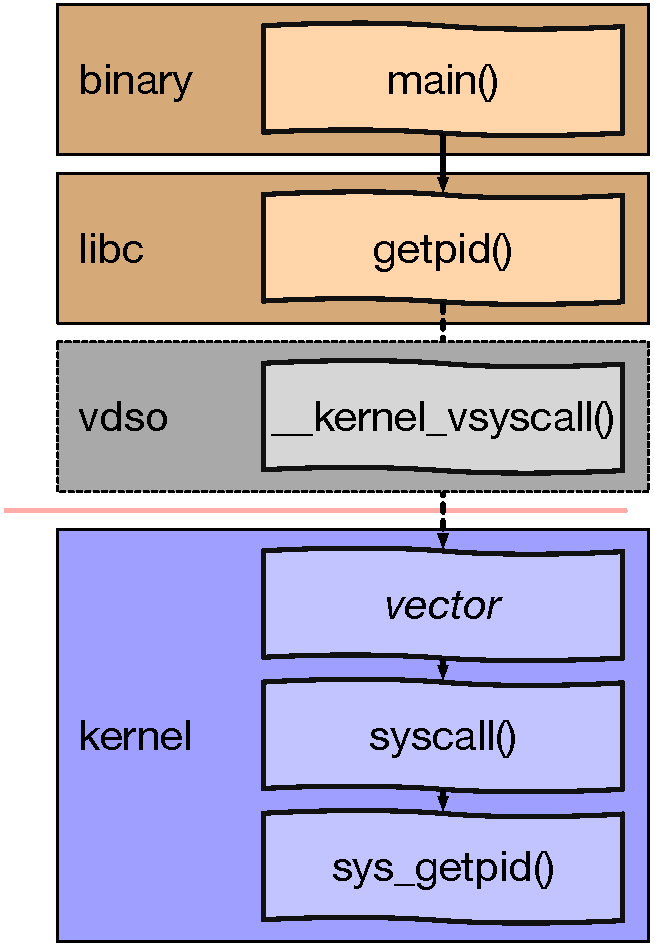
\includegraphics[width=\textwidth]{../../figures/syscall-stacks.pdf}

    \pause

    \column{0.6\textwidth}
      \begin{itemize}
	\item \texttt{libc} system-call function stubs provide linkable
	  symbols
	\item Stubs inline system-call instructions, or use dynamic
	  implementations
	\begin{itemize}
	  \item Linux, FreeBSD \texttt{vdso}
	  \item Xen hypercall page
	\end{itemize}

	\pause
	\medskip

	\item Low-level vector calls \texttt{syscall()}
	\begin{itemize}
	  \item System-call prologue runs \\
	    (e.g., breakpoints, tracing)
	  \item Actual kernel service invoked
	  \item System-call epilogue runs \\
	    (e.g., more tracing, signal delivery)
	\end{itemize}
      \end{itemize}
  \end{columns}
\end{frame}

\begin{frame}[fragile]
  \frametitle{The system-call table: \texttt{syscalls.master}}

  \begin{scriptsize}
\begin{verbatim}
...
33  AUE_ACCESS    STD     { int access(char *path, int amode); }
34  AUE_CHFLAGS   STD     { int chflags(const char *path, u_long flags); }
35  AUE_FCHFLAGS  STD     { int fchflags(int fd, u_long flags); }
36  AUE_SYNC      STD     { int sync(void); }
37  AUE_KILL      STD     { int kill(int pid, int signum); }
38  AUE_STAT      COMPAT  { int stat(char *path, struct ostat *ub); }
...
\end{verbatim}
  \end{scriptsize}

  \pause

  \begin{center}
    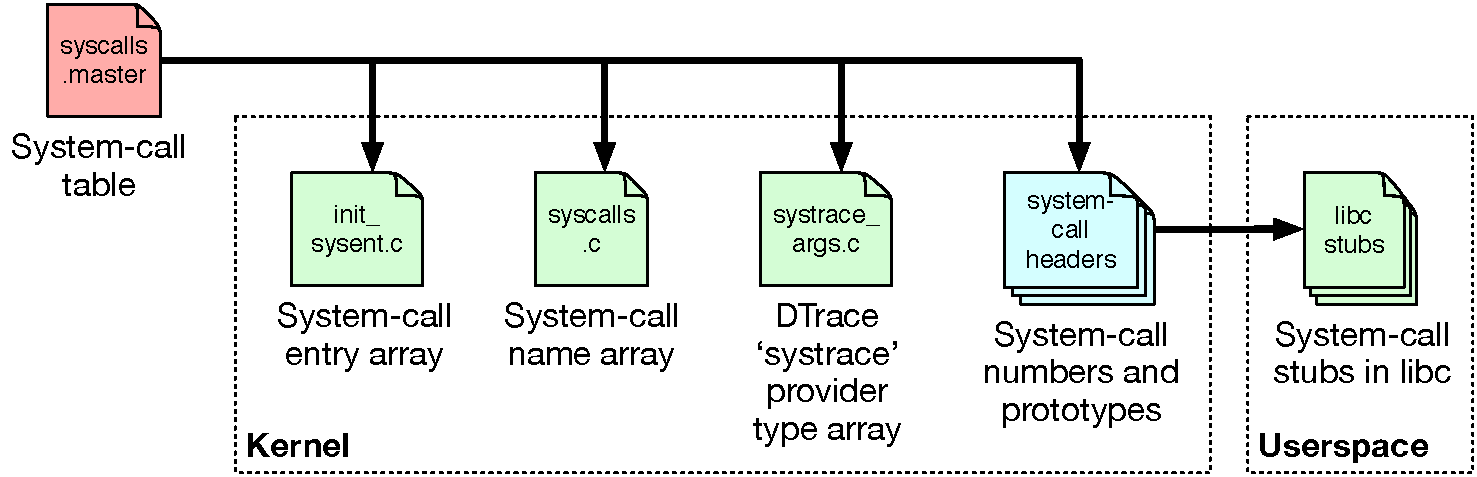
\includegraphics[width=0.9\textwidth]{../../figures/syscall-table-output.pdf}
  \end{center}

  \pause

  NB: If this looks like RPC stub generation .. that's because it is.
\end{frame}

\begin{frame}
  \frametitle{Security and reliability}

  \begin{itemize}
    \item Kernel interface is key \textit{Trusted Computing Base} (TCB)
      surface
    \begin{itemize}
      \item ``Minimum software required for the system to be secure''
    \end{itemize}

    \pause
    \medskip

    \item Foundational security goal: \textit{isolation}
    \begin{itemize}
      \item \textit{Integrity}, \textit{confidentiality}, \textit{availability}

      \pause

      \item Limit scope of effects of calls
      \item Enforce access control on all operations (e.g., DAC)
      \item Accountability mechanisms (e.g., event auditing)
    \end{itemize}

    \pause
    \medskip

    \item System calls perform work on behalf a user thread
    \begin{itemize}
      \item Credential \textit{unforgeably} tied to process/threads
      \item Thread credential authorises work kernel performs
      \item Resources (e.g., CPU, memory) billed to the thread
      %\item Debugging/profiling information exposed to the thread's owner
    \end{itemize}

    \pause
    \medskip

    \item Kernel must be robust to user-thread misbehaviour
    \begin{itemize}
      \item Handle failures gracefully: terminate process, not kernel
      \item Avoid priority inversions, unbounded resource allocation, etc.
    \end{itemize}

  \end{itemize}
\end{frame}

\begin{frame}
  \frametitle{Security and reliability (cont)}

  \begin{itemize}
    \item Confidentiality is both hard and expensive
    \begin{itemize}
      \item Explicitly zero memory before re-use between security domains
      \item Prevent kernel-user data leaks (e.g., in structure padding)
      \item Be aware of \textit{covert channels}, \textit{side channels}
    \end{itemize}

    \pause
    \medskip

    \item User code is the adversary -- may try to break isolation
    \begin{itemize}
      \item Kernel must carefully enforce all access-control rules
      \item System-call arguments and return values are data, not code
      \item Extreme care with user-originated pointers
    \end{itemize}

    \pause
    \medskip

    \item User passes kernel pointer to system call
    \begin{itemize}
      \item System-call arguments must be processed with rights of user code

      \pause
      \smallskip

      \item E.g., prohibit \texttt{read()} from passing kernel pointer so
	that in-kernel credentials can be overwritten
      \item Explicit \texttt{copyin()}, \texttt{copyout()} check pointer
	validity, copy data
    \end{itemize}

    \pause
    \medskip

    \item Kernel dereferences user pointer by accident
    \begin{itemize}
      %\item Asymmetry: kernel can access user memory, but not vice versa
      \item Kernel bugs could cause kernel to access user memory by mistake

      \pause
      \smallskip

      \item Kernel \texttt{NULL}-pointer vulnerabilities
      \item Intel Supervisor Mode Access Prevention (SMAP)
    \end{itemize}
  \end{itemize}
\end{frame}

\begin{frame}
  \frametitle{System-call entry -- the guts: \texttt{syscallenter}}

  \begin{tabular}{ll}
  \texttt{cred\_update\_thread} & Update thread cred from process \\

  \pause

  \texttt{sv\_fetch\_syscall\_args} & ABI-specific \texttt{copyin()} of
      arguments \\

  \pause

  \texttt{ktrsyscall} & \texttt{ktrace} syscall entry \\

  \pause

  \texttt{ptracestop} & \texttt{ptrace} syscall entry breakpoint \\

  \pause

  \texttt{IN\_CAPABILITY\_MODE} & Capsicum capability-mode check \\

  \pause

  \texttt{syscall\_thread\_enter} & Thread drain barrier (module unload) \\

  \pause

  \texttt{systrace\_probe\_func} & DTrace system-call entry probe \\

  % I've never understood why the skips are where they are in tabulars
  \medskip
  \pause

  \texttt{AUDIT\_SYSCALL\_ENTER} & Security event auditing \\

  \medskip
  \pause

  \texttt{sa->callp->sy\_call} & \textbf{System-call implementation!  Woo!} \\

  \pause

  \texttt{AUDIT\_SYSCALL\_EXIT} & Security event auditing \\

  \pause

  \texttt{systrace\_probe\_func} & DTrace system-call return probe \\

  \pause

  \texttt{syscall\_thread\_exit} & Thread drain barrier (module unload) \\

  \pause

  \texttt{sv\_set\_syscall\_retval} & ABI-specific return value \\
  \end{tabular}

  \pause
  \begin{itemize}
    \item That's a lot of tracing hooks -- why so many?
  \end{itemize}
\end{frame}

\begin{frame}[fragile]
  \frametitle{\texttt{getauid}: return process audit ID}

  \begin{scriptsize}
\begin{verbatim}
int
sys_getauid(struct thread *td, struct getauid_args *uap)
{
        int error;

        if (jailed(td->td_ucred))
                return (ENOSYS);
        error = priv_check(td, PRIV_AUDIT_GETAUDIT);
        if (error)
                return (error);
        return (copyout(&td->td_ucred->cr_audit.ai_auid, uap->auid,
            sizeof(td->td_ucred->cr_audit.ai_auid)));
}
\end{verbatim}
  \end{scriptsize}

  \begin{itemize}
    \item Current thread, system-call argument structure
    \begin{itemize}
      \item Security checks: lightweight virtualisation, privilege
      \item Copy value to user address space -- can't write to it directly!
      \item No synchronisation as all fields thread-local
    \end{itemize}

    \pause

    \item Does it matter how fresh the credential pointer is?
  \end{itemize}
\end{frame}

\begin{frame}
  \frametitle{System-call return -- the guts: \texttt{syscallret}}

  \begin{tabular}{ll}
  \texttt{userret} & Complicated things like signals \\

  \pause
  $\rightarrow$
    \texttt{KTRUSERRET} & \texttt{ktrace} syscall return \\

  \pause

  $\rightarrow$
    \texttt{g\_waitidle} & Wait for disk probe to settle \\

  \pause

  $\rightarrow$
    \texttt{addupc\_task} & System-time profiling charge \\

  \pause

  $\rightarrow$
    \texttt{sched\_userret} & Scheduler adjusts priority \\

  \pause
  \medskip

  & {... various debugging assertions ...} \\

  \pause

  \texttt{p\_throttled} & \texttt{racct} resource throttling \\

  \pause

  \texttt{ktrsysret} & Kernel tracing: syscall return \\

  \pause

  \texttt{ptracestop} & \texttt{ptrace} syscall return breakpoint \\

  \pause

  \texttt{thread\_suspend\_check} & Single-threading check \\

  \pause

  \texttt{P\_PPWAIT} & \texttt{vfork} wait \\
  \end{tabular}

  \pause
  \medskip

  \begin{itemize}
    \item That is a lot of stuff that largely \textbf{never happens}
    \item The trick is making all this nothing fast -- e.g., via a small
      number of per-thread flags and globals that remain in the cache
  \end{itemize}
\end{frame}

%\begin{frame}
%  \frametitle{Should I add a new system call?}
%
%  XXX: How did we get all these system calls? \\
%  XXX: The tradeoff space \\
%  XXX: Does it need to be in the kernel? \\
%  XXX: Should it be a device node? \\
%  XXX: FreeBSD: should it be a sysctl? \\
%  XXX: Linux: should it be a new filesystem and/or procfs/sysfs node? \\
%  XXX: Even then, some confusion: ACLs vs extended attributes
%
%\end{frame}

\begin{frame}[fragile]
  \frametitle{System calls in practice: \texttt{dd}}

  \begin{scriptsize}
\begin{verbatim}
# time dd if=/dev/zero of=/dev/null bs=10m count=1 status=none
0.000u 0.396s 0:00.39 100.0%	25+170k 0+0io 0pf+0w
\end{verbatim}
  \end{scriptsize}

  \pause

  \begin{scriptsize}
\begin{verbatim}
syscall:::entry /execname == "dd"/ {
        self->start = timestamp;
        self->insyscall = 1;
}

syscall:::return /execname == "dd" && self->insyscall != 0/ {
        length = timestamp - self->start;
        @syscall_time[probefunc] = sum(length);
        @totaltime = sum(length);
        self->insyscall = 0;
}

END {
        printa(@syscall_time);
        printa(@totaltime);
}
\end{verbatim}
  \end{scriptsize}
\end{frame}

\begin{frame}[fragile]
  \frametitle{System calls in practice: \texttt{dd} (2)}

  \begin{scriptsize}
\begin{verbatim}
# time dd if=/dev/zero of=/dev/null bs=10m count=1 status=none
0.000u 0.396s 0:00.39 100.0%    25+170k 0+0io 0pf+0w
\end{verbatim}
  \end{scriptsize}

  \pause

  \begin{scriptsize}
\begin{verbatim}
  sysarch                                                        7645
  issetugid                                                      8900
  lseek                                                          9571
  sigaction                                                     11122
  clock_gettime                                                 12142
  ioctl                                                         14116
  write                                                         29445
  readlink                                                      49062
  access                                                        50743
  sigprocmask                                                   83953
  fstat                                                        113850
  munmap                                                       154841
  close                                                        176638
  lstat                                                        453835
  openat                                                       562472
  read                                                         697051
  mmap                                                         770581
          3205967
\end{verbatim}
  \end{scriptsize}

  \pause

  NB: $\approx$ 3.2ms total -- but \texttt{time(1)} reports 396ms system time?
\end{frame}

\begin{frame}[fragile]
  \frametitle{Traps in practice: \texttt{dd} (1)}

  \begin{tiny}
\begin{verbatim}
syscall:::entry /execname == "dd"/ {
        @syscalls = count();
        self->insyscall = 1;
        self->start = timestamp;
}

syscall:::return /execname == "dd" && self->insyscall != 0/ {
        length = timestamp - self->start; @syscall_time = sum(length);
        self->insyscall = 0;
}

fbt::trap:entry /execname == "dd" && self->insyscall == 0/ {
        @traps = count(); self->start = timestamp;
}

fbt::trap:return /execname == "dd" && self->insyscall == 0/ {
        length = timestamp - self->start; @trap_time = sum(length);
}

END {
        printa(@syscalls); printa(@syscall_time);
        printa(@traps); printa(@trap_time);
}
\end{verbatim}
  \end{tiny}

  \pause

  \begin{tiny}
\begin{verbatim}
               65
          2953756
             5185
        380762894
\end{verbatim}
  \end{tiny}

  \pause

  NB: 65 system calls at $\approx$3ms; 5185 traps at $\approx$381ms!  But
    which traps?
\end{frame}

\begin{frame}[fragile]
  \frametitle{Traps in practice: \texttt{dd} (1)}

  \begin{scriptsize}
\begin{verbatim}
profile-997 /execname == "dd"/ { @traces[stack()] = count(); }
\end{verbatim}
  \end{scriptsize}

  \pause

  \begin{scriptsize}
\begin{verbatim}
...
              kernel`PHYS_TO_VM_PAGE+0x1
              kernel`trap+0x4ea
              kernel`0xffffffff80e018e2
                5

              kernel`vm_map_lookup_done+0x1
              kernel`trap+0x4ea
              kernel`0xffffffff80e018e2
                5

              kernel`pagezero+0x10
              kernel`trap+0x4ea
              kernel`0xffffffff80e018e2
              346
\end{verbatim}
  \end{scriptsize}

  \pause

  \begin{itemize}
  \item A sizeable fraction of time is spent in \texttt{pagezero}: on-demand
    zeroing of previously untouched pages

  \item Ironically, the kernel is filling pages with zeroes only to
    immediately \texttt{copyout()} zeros to it from \texttt{/dev/zero}
  \end{itemize}

\end{frame}

\section{Revisiting virtual memory}

\begin{frame}
  \frametitle{So: back to virtual memory (VM)}

  \begin{itemize}
    \item The process model's isolation guarantees incur real expenses

    \medskip
    \pause

    \item But the virtual-memory subsystem works quite hard to avoid them
    \begin{itemize}
      \item \textit{Shared memory}, \textit{copy-on-write}, \textit{page
	flipping}
      \item Background page zeroing
      \item Superpages to improve TLB efficiency
    \end{itemize}

    \medskip
    \pause

    \item VM optimisation avoids work, but also manages memory footprint
    \begin{itemize}
      \item Memory as a \textit{cache} of secondary storage (files, swap)
      \item Demand paging vs. I/O clustering
      \item LRU / Preemptive swapping/paging to maintain free page pool
      \item Memory compression and deduplication
    \end{itemize}

    \medskip
    \pause

    \item These ideas were known before Mach, but ...
    \begin{itemize}
      \item Acetta, et al turn them into an art form
      \item Provide a \textit{model} beyond V$\rightarrow$P mappings in page
	tables
      \item And ideas such as the \textit{message-passing--shared-memory
	duality}
    \end{itemize}
  \end{itemize}
\end{frame}

\begin{frame}
  \frametitle{Last time: virtual memory (quick but painful primer)}

  \begin{center}
    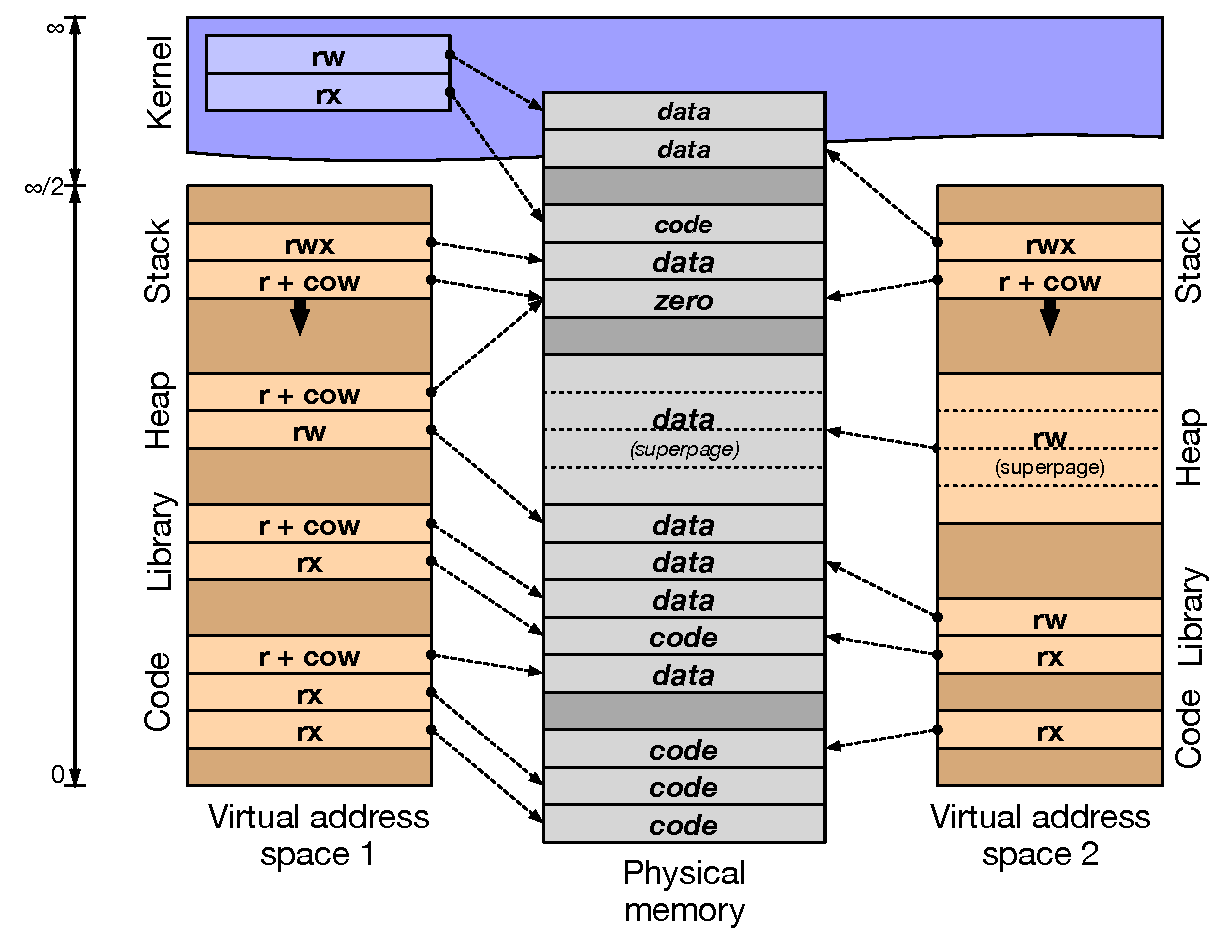
\includegraphics[width=0.8\textwidth]{../../figures/process-address-space.pdf}
  \end{center}
\end{frame}

\begin{frame}
  \frametitle{A (kernel) programmer model for virtual memory}

  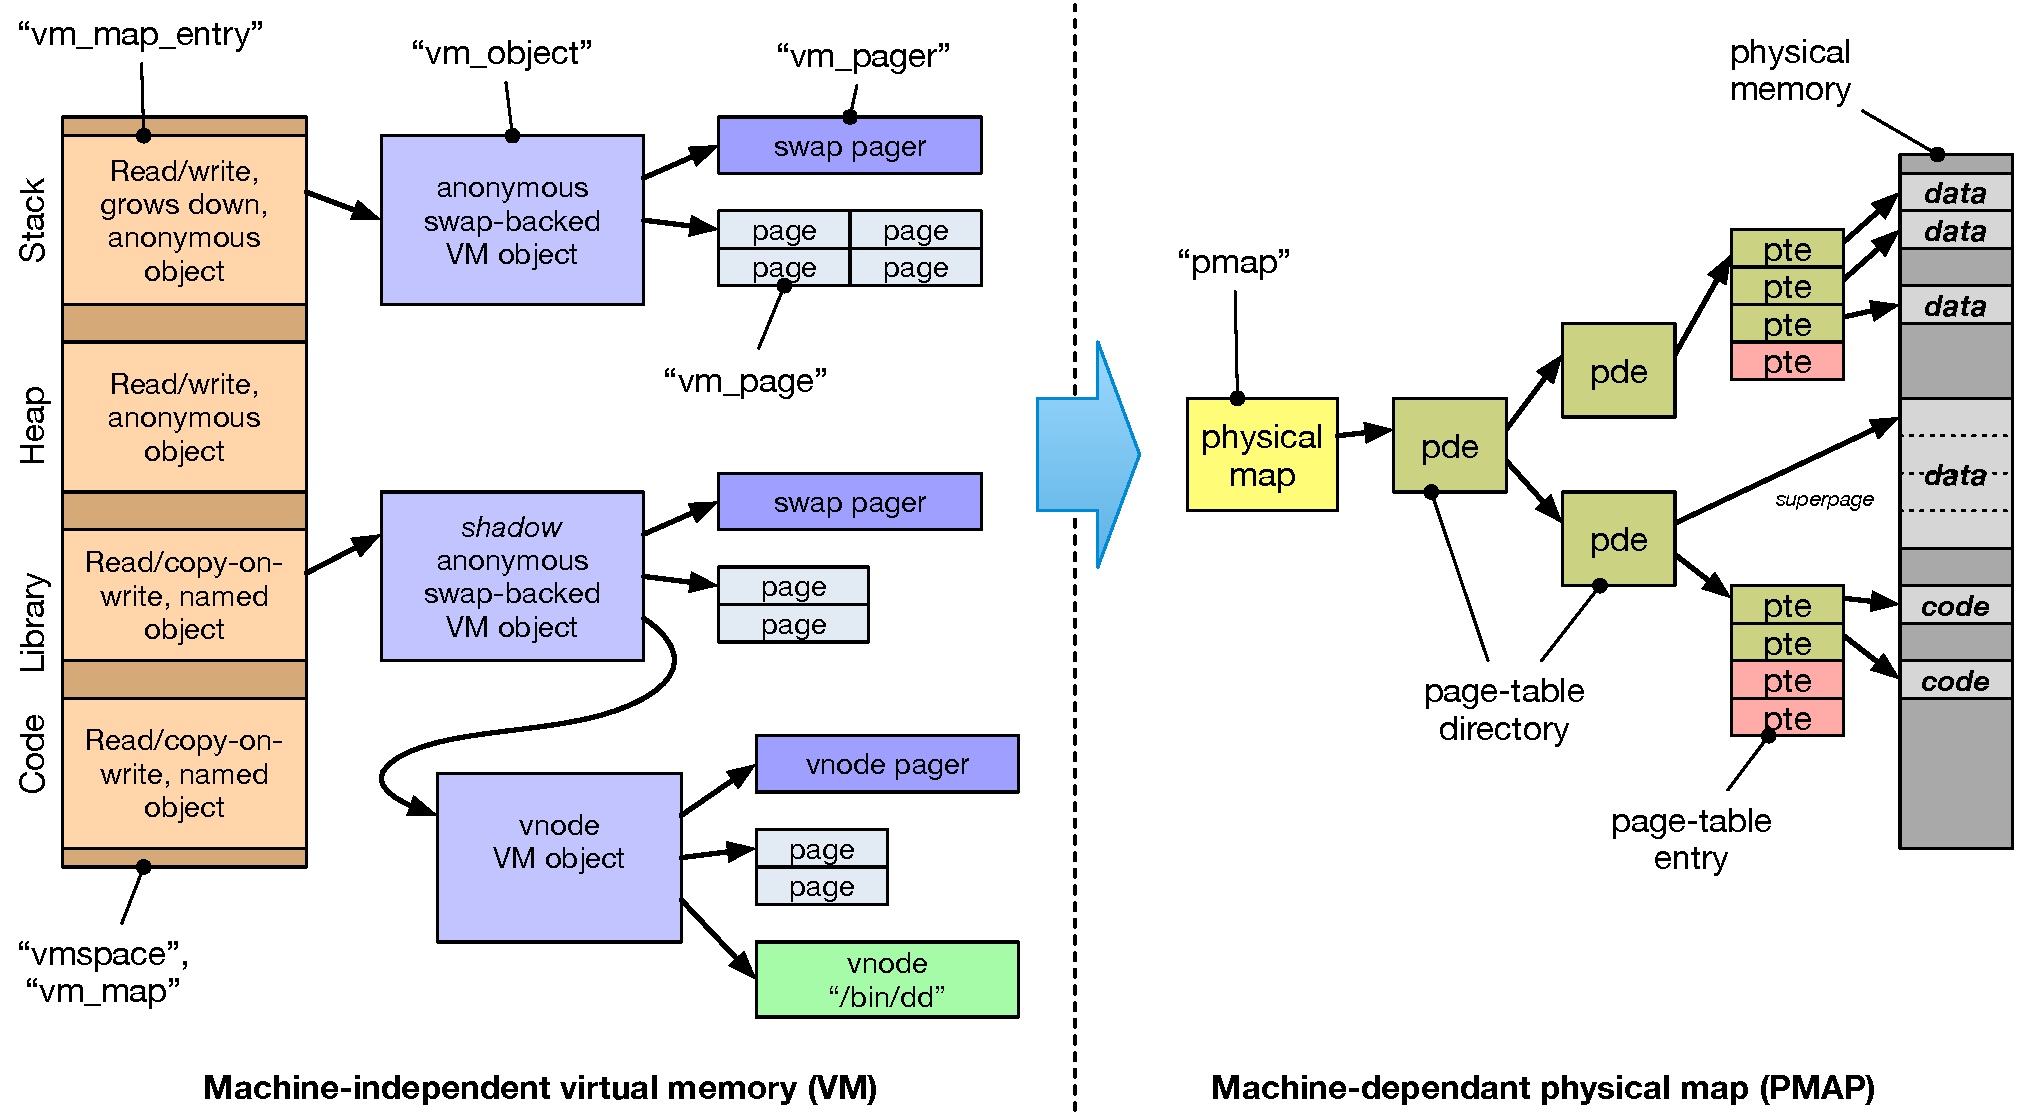
\includegraphics[width=\textwidth]{../../figures/mach-vm-model.pdf}
\end{frame}

%
% This is where we'd want to put a slide on how the VM system is largely
% driven by page faults in order to be as lazy as possible.
%

\begin{frame}
  \frametitle{Mach VM in other operating systems}

  \begin{itemize}
    \item In Mach, VM mappings, objects, pages, etc, were first-class objects
      exposed to userspace via system calls

    \medskip
    \pause

    \item In two directly derived systems, quite different stories:
    \begin{description}
      \item[Mac OS X] Although XNU is not a microkernel, Mach's VM/IPC APIs
	are visible to applications, and used frequently
      \item[FreeBSD] Mach VM is used as a foundation and are only available as
	a Kernel Programming Interface (KPI)
    \end{description}

    \medskip
    \pause

    \item In FreeBSD, Mach VM KPIs are used:
    \begin{itemize}
      \item To efficiently implement UNIX's \texttt{fork()} and
	\texttt{execve()}
      \item For memory-management APIs such as \texttt{mmap()} and
	\texttt{mprotect()}
      \item By the filesystem to implement a merged VM-buffer cache
      \item By device drivers that manage memory in interesting ways (e.g.,
	GPU drivers mapping pages into user processes)
      \item By a set of VM worker threads, such as the \textit{page daemon},
	\textit{swapper}, \textit{syncer}, and page-zeroing thread
    \end{itemize}
  \end{itemize}
\end{frame}

\section{Conclusion}

\begin{frame}
  \frametitle{For next time}

  \begin{itemize}
    \item The second lab: DTrace and I/O
    \item Begin to explore Inter-Process Communication (IPC) performance

    \bigskip

    \item Ellard and Seltzer 2003
  \end{itemize}

  \bigskip

  \textbf{If you are having trouble getting hold of the course texts:} Please
    ask the department librarian or your college librarian to order copies.

\end{frame}

\end{document}
